\documentclass{article}
\usepackage{amsmath}
\usepackage{hyperref}
\usepackage{url}
\usepackage{amssymb}
\usepackage{graphicx}
\usepackage{float}
\usepackage{bm}
\usepackage[top=2cm]{geometry}
\renewcommand{\thesubsubsection}{\thesubsection\ \alph{subsubsection})}

\title{Deep Learning - Homework 2}
\author{99222 - Frederico Silva, 99326 - Sebastião Carvalho}
\date{\today}

\begin{document}

\maketitle

\tableofcontents

\section{Question 1}

\subsection{Question 1.1}

Using a single attention head, the output $Z$ is given by:

\begin{equation}
    Z = \text{softmax} \left( \frac{QK^T}{\sqrt{d_k}} \right) V
\end{equation}

The complexity of computing this $Z$ is the complexity of computing all the matrix multiplications and the softmax.

Starting with the dimensions of each matrix, we have:
$
    Q \in \mathbb{R}^{L \times D}, K \in \mathbb{R}^{L \times D}, V \in \mathbb{R}^{L \times D}
$

\bigskip

The complexity of computing a matrix product $AB$ where $A \in \mathbb{R}^{m \times n}$ and $B \in \mathbb{R}^{n \times p}$ is $O(mnp)$.
We can prove this since to compute the element $c_{ij}$ of the matrix $C = AB$ we need to compute the dot product of the $i$-th row of 
$A$ with the $j$-th column of $B$, and this dot product has complexity $O(n)$, because it is the sum of $n$ products of real numbers.
Since we need to compute $mn$ elements of $C$, the complexity of computing $C$ is $O(mnp)$.

\bigskip

Let's consider $P = softmax \left( \frac{QK^T}{\sqrt{d_k}} \right)$. With this $P$ we can compute $Z = PV$.

In our case, we first need to compute $QK^T$ and since $Q \in \mathbb{R}^{L \times D}$ and $K^T \in \mathbb{R}^{D \times L}$, 
the complexity of this operation is $O(L^2D)$.

Then, we need to divide each element of $QK^T$ by $\sqrt{d_k}$, which has complexity $O(L^2)$.
Finally, we need to compute the softmax of each row of the matrix $QK^T / \sqrt{d_k}$, which has complexity $O(L^2)$.
The complexity of computing $P$ is $O(L^2D + L^2 + L^2) = O(L^2D)$. 
Since $P = softmax \left( \frac{QK^T}{\sqrt{d_k}} \right)$, $P \in \mathbb{R}^{L \times L}$.

\bigskip

Lastly we need to compute the matrix product $PV$. Since $P \in \mathbb{R}^{L \times L}$ and $V \in \mathbb{R}^{L \times D}$,
the complexity of this operation is $O(L^2D)$.

With this the final complexity of computing $Z$ is $O(L^2D)$, since the complexity of computing $P$ is $O(L^2D)$ 
and the complexity of computing $PV$ is $O(L^2D)$.

\bigskip

Let's consider the numebr of hidden units (D) is fixed, so the complexity of computing $Z$ is $O(L^2)$.

This may cause a problem for long sequences of text, since the complexity of computing $Z$ is $O(L^2)$, where $L$ is the length of the sequence.
This means that the complexity of computing $Z$ is quadratic in the length of the sequence, which is not good for long sequence inputs.

\subsection{Question 1.2}

For this exercise we will use the McLaurin series expansion of the exponential function to approximate the softmax and reduce the computational 
computational complexity. The McLaurin series expansion of the exponential function is given by:

\bigskip

$exp(t) = \sum_{n=0}^{\infty} \frac{t^n}{n!}$

\bigskip

First, considering $exp(t) \approx 1 + t + \frac{t^2}{2}, $ we want to create a feature map $\phi: \mathbb{R}^D \rightarrow \mathbb{R}^M$ such that, 
for arbitrary $q \in \mathbb{R}^D$ and $k \in \mathbb{R}^D$ we have $exp(q^Tk) \approx \phi(q)^T \phi(k)$.

With this, we want to find a mapping $\phi$ such that:
$ \phi(q)^T \phi(k) = 1 + q^Tk + \frac{(q^Tk)^2}{2} $

\bigskip

The first two terms of the series are trivial, since we can define $\phi(q) = [1, q_1, \dots, q_n]$. 
For the third term, we need to decompose the square of the dot product of $q$ and $k$ into a sum of products of the elements of $q$ and $k$.

For vectors $x$ and $z$ with the same dimension $n$, we have that $x^Tz = \sum_{i=1}^{D} x_iz_i$.
Now for the square of the doct product we have:

\medskip

$ (x^Tz)^2 = (x_1z_1 + \dots + x_n)(x_1z_1 + \dots + x_nz_n) = \\
(x_1z_1)^2 + 2x_1z_1x_2z_2 + \dots + 2x_1z_1x_nz_n + \\
+ (x_2z_2)^2 + \dots + x_2z_2x_nz_n + \\
\dots + \\
 (x_nz_n)^2 = \\
\sum_{i=1}^n (x_i)^2(z_i)^2 + 2\sum_{i=1}^{n-1} \sum_{j=i+1}^{n} x_iz_ix_jz_j \\
$

This way we can define $\phi(x) = [1, x_1, \dots, x_n, 
\frac{1}{\sqrt{2}}x_1^{2}, x_1x_2, \dots, x_1x_n, \frac{1}{\sqrt{2}}x_2^{2}, \dots, 
x_2x_n, \dots, x_{n-1}x_n , \frac{1}{\sqrt{2}}x_n^{2}]$

With this $exp(q^Tk) \approx \phi(q)^T \phi(k)$, and we can use this to approximate the softmax function.

\bigskip

In terms of dimensionality, if the vector $x$ has dimension $D$, the first two terms of the series will have dimension $D + 1$. From the 
third term, we can see that the number of terms will be $\sum_{i=1}^{D} i = \frac{D(D+1)}{2}$. With this, for $K = 2$, 
the vector $\phi(x)$ will have dimension $M = 1 + D + \frac{D(D+1)}{2}$.

\bigskip

Now we want to acess what would be the dimensionality of the feature space $M$ if we used the McLaurin series with $K \geq 3$ terms.
For this, we have to acess the dimensionality of each term.

\bigskip

According to the multinomial theorem:

\medskip

$ (x_1 + x_2 + \dots + x_D)^K = \sum_{k_1 + k_2 + \dots + k_D = K, k_1, k_2, \dots, k_D\geq0} \binom{n}{k_1, k_2, \dots, k_D} \prod_{t=1}^D x_t^{k_t}$

where $\binom{n}{k_1, k_2, \dots, k_D} = \frac{n!}{k_1!k_2!\dots k_D!}$

\bigskip

According to this theorem, the number of multinomial coefficients is given by $\binom{K + D - 1}{D - 1}$, and thus, the number of terms in the expansion for the $K-th$ is
$\binom{K + D - 1}{D - 1}$.

\bigskip

With this, for $K \geq 3$, the dimensionality of the feature space will be:

$M = \sum \binom{K + D - 1}{D - 1}$

\subsection{Question 1.3}

In the previous exercise, we defined the feature map $\phi: \mathbb{R^D} \rightarrow \mathbb{R^M}$, such that $exp(q^Tk) \approx \phi(q)^T\phi(k)$. 
Now let's consider the mapping $\Phi$ where $\Phi(X)$, which results in a matrix whose rows are $\phi(x_i)$, where $x_i$ is the $i$-th row of $X$.

Our goal is to show that the self-attention operation can be approximated as $Z \approx D^{-1}\Phi(Q) \Phi(K)^T V$, 
where $D = Diag(\Phi(Q) \Phi(K)^T 1_L)$. 

Looking at the original self-attention operation, we can see that the diffence is that now we want to approximate
$softmax(QK^T)$ as $D^{-1}\Phi(Q) \Phi(K)^T$.

Considering $softmax(QK^T)_{ij} = \frac{exp(q_i^Tk_j)}{\sum_{l=1}^L exp(q_i^Tk_l)}$, since we want
$softmax(QK^T) \approx D^{-1}\Phi(Q) \Phi(K)^T$, we can see that $D^{-1}$ will correspond to the denominator of the softmax operation,
and $\Phi(Q) \Phi(K)^T$ will correspond to the numerator.

\bigskip

Let's focus on the $\Phi(Q) \Phi(K)^T$ part. We know that this is the same as:

\medskip

$
    \Phi(Q) \Phi(K)^T = 
    \begin{bmatrix}
        --- \phi(q_1) --- \\
        --- \phi(q_2) --- \\
        \vdots \\
        --- \phi(q_L) --- \\
    \end{bmatrix}
    \begin{bmatrix}
        | & | & \dots & | \\
        \phi(k_1) & \phi(k_2) & \dots & \phi(k_L) \\
        | & | & \dots & | \\
    \end{bmatrix}
$

\medskip

Since $\phi(q_i)$ is spread along the $i$-th row, for the $(i,j)$-th element of the matrix $\Phi(Q) \Phi(K)^T$ we have that cell $i,j$ is equal to $
phi(q_i)_1 \phi(k_j)_1 + phi(q_i)_2 \phi(k_j)_2 + \dots + phi(q_i)_M \phi(k_j)_M = \phi(q_i)^T \phi(k_j)$.

With this we can see that $\Phi(Q) \Phi(K)^T$ is a matrix whose $(i,j)$-th element is $\phi(q_i)^T \phi(k_j)$.

We know that $\phi(q)^T\phi(k) \approx exp(q^Tk)$, so we can see that $\Phi(Q) \Phi(K)^T$ is a matrix whose $(i,j)$-th element is an 
approximation $exp(q_i^Tk_j)$.

\bigskip

Now let's look at $D$. We know that $D = Diag(\Phi(Q) \Phi(K)^T 1_L)$. Since $\Phi(Q) \Phi(K)^T$ is a matrix whose $(i,j)$-th element is an
approximation $exp(q_i^Tk_j)$, and $1_L$ is a vector of ones, the product $\Phi(Q) \Phi(K)^T 1_L$ will be a vector whose $i$-th element
is an approximation of $\sum_{j=1}^L exp(q_i^Tk_j)$, since it is the sum of the $i$-th row of $\Phi(Q) \Phi(K)^T$.

With this, we can see that $D \in \mathbb{R}^{L\times L}$ is a diagonal matrix whose $(i, i)$-th element is an approximation of $\sum_{j=1}^L exp(q_i^Tk_j)$.
Since this is a diagonal matrix, and the inverse of a diagonal matrix is a diagonal matrix whose $(i, i)$-th element is the inverse of the $(i, i)$-th element
we can see that $D^{-1}$ is a diagonal matrix whose $(i, i)$-th element is an approximation of $\frac{1}{\sum_{j=1}^L exp(q_i^Tk_j)}$.

\bigskip

Now that we have $D^{-1}$ and $\Phi(Q) \Phi(K)^T$, we can see that $D^{-1}\Phi(Q) \Phi(K)^T$ is a matrix whose $(i,j)$-th element is an approximation of
the softmax operation, which is what we wanted to show. With this, we can see that $Z = softmax(QK^T)V \approx D^{-1}\Phi(Q) \Phi(K)^T V$.

\subsection{Question 1.4}

\section{Question 2}

\subsection{Question 2.1}
After running the code, the best configuration was for the learning rate of 0.01.
The following plots were generated:

\begin{figure}[H]
    \centering
    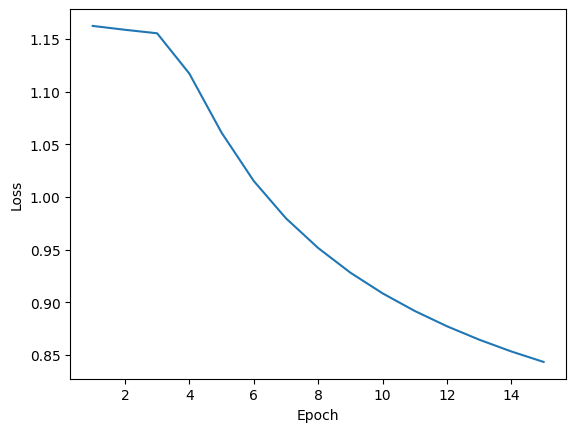
\includegraphics[width=0.8\textwidth]{plots/CNN-training-loss-0.01-0.7-0-sgd-False.png}
    \caption{Training loss for $\eta=0.01$}
    \label{fig:2.1-training_loss}
\end{figure}

\begin{figure}[H]
    \centering
    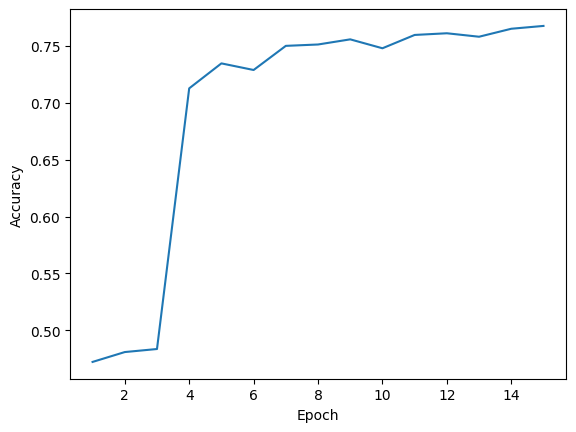
\includegraphics[width=0.8\textwidth]{plots/CNN-validation-accuracy-0.01-0.7-0-sgd-False.png}
    \caption{Validation accuracy for $\eta=0.01$}
    \label{fig:2.1-validation_accuracy}
\end{figure}

The final test accuracy was 0.8280.

\subsection{Question 2.2}
The performance of this network was slightly worse than the previous one, 
having achieved a final test accuracy of 0.8147.

\subsection{Question 2.3}
Both network present the same number of parameters, 224892.
The difference in performance between the two networks, resides in the use 
of max pooling layers. Max pooling can help the network focusing on the most
important features, making the network more robust to small changes in the
input. Furthermore, max pooling can also help with overfitting. In our case, 
the use of max pooling layers helped the network to achieve a better test 
accuracy results.

\section{Question 3}

\subsection{Question 3.1}

\subsection{Question 3.2}

\subsection{Question 3.3}

\subsection{Question 3.4}

\section{Credits}

\section{Sources}

\begin{itemize}
    \item \href{https://www.educative.io/answers/what-is-a-max-pooling-layer-in-cnn}{What is a max pooling layer in CNN?}
\end{itemize}

\end{document}